\documentclass[a4paper,11pt]{article}
\usepackage[margin=3cm]{geometry}
\linespread{1.25}

\usepackage[T1]{fontenc}
\usepackage[utf8]{inputenc}
% \usepackage[swedish]{babel}
% \usepackage{fontspec}
% \setmainfont{Linux Libertine O}
\usepackage{lmodern}
\usepackage{graphicx}
\usepackage{float}

\usepackage{fancyhdr}
\pagestyle{fancy}
\renewcommand{\headrulewidth}{ 1.0pt }
\renewcommand{\footrulewidth}{ 0.4pt }
\fancyhead{} % clear all headers
\fancyfoot{} % clear all footers

% E:even page, O:odd page, L:left, C:center, R:right
%\fancyhead[LE,RO]{\thepage}
%\fancyfoot[C]  {Albert Einstein, 2009}

\fancyhead[L]{DH2323 (DGI17) Lab 1}
\fancyhead[R]{Mikael Forsberg, Robin Gunning}
\fancyfoot[C]{\thepage}

\begin{document}
\title{\vspace{-2cm} Lab 1: Setup, 2D Graphics Intro and Starfield\\ \small DH2323 (DGI17)\\ KTH Royal Institute of Technology}
\author{Mikael Forsberg <miforsb@kth.se>\\ Robin Gunning <rgunning@kth.se>}
\maketitle

\vspace{-1.25cm}

\section*{Overview}
We completed all the given tasks and also added motion blur.

\section*{Setup of the Lab Environment}
We both use modern Debian GNU/Linux systems, and after a quick
\texttt{apt-get install libsdl1.2-dev} we were able to \texttt{cmake .} and \texttt{make}
the skeleton code. Neither of us used an IDE for any of the coding in the course, instead
sticking to the tried and true text editor + terminal combo.

\section*{Introduction to 2D Computer Graphics}
The instructions for the task of bilinear interpolation felt a bit disorganized. Section 2.2
starts by talking about replicating the rainbow image seen earlier, but this turns out not to be
the topic of the section itself. Having all discussion of bilinear interpolation in section 2.3
would have been better, and having an image to illustrate the idea would have been nice.

That said, this task was simple to implement and we got the expected result:

\begin{figure}[H]
\begin{center}
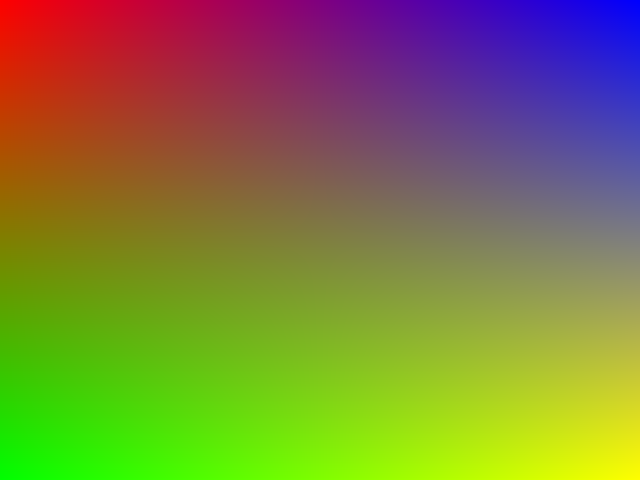
\includegraphics[width=5cm]{bilinear.png}
\caption{Bilinear interpolation}
\end{center}
\end{figure}
\vspace{-1.5cm}

\section*{Starfield}
Sections 3.0 and 3.1 were straightforward and got us to an unimpressive view of randomly placed
white dots that were initially so tiny that we decided to draw four pixels
([x,y], [x+1,y], [x,y+1], [x+1,y+1]) instead of just one for each star:

\begin{figure}[H]
\begin{center}

\includegraphics[width=12cm]{stars.png}
\caption{Randomly placed stars drawn with perspective projection}
\end{center}
\end{figure}
\vspace{-0.5cm}

\noindent
Section 3.2 was also straightforward, but because we had changed the window size to a 16:9 aspect
ratio there were visibly less stars towards the left and right edges of the screen. To fix this we
changed the initialization of the $x$ coordinates of stars to have a range of $[-1.5, 1.5]$.

\begin{figure}[H]
\begin{center}
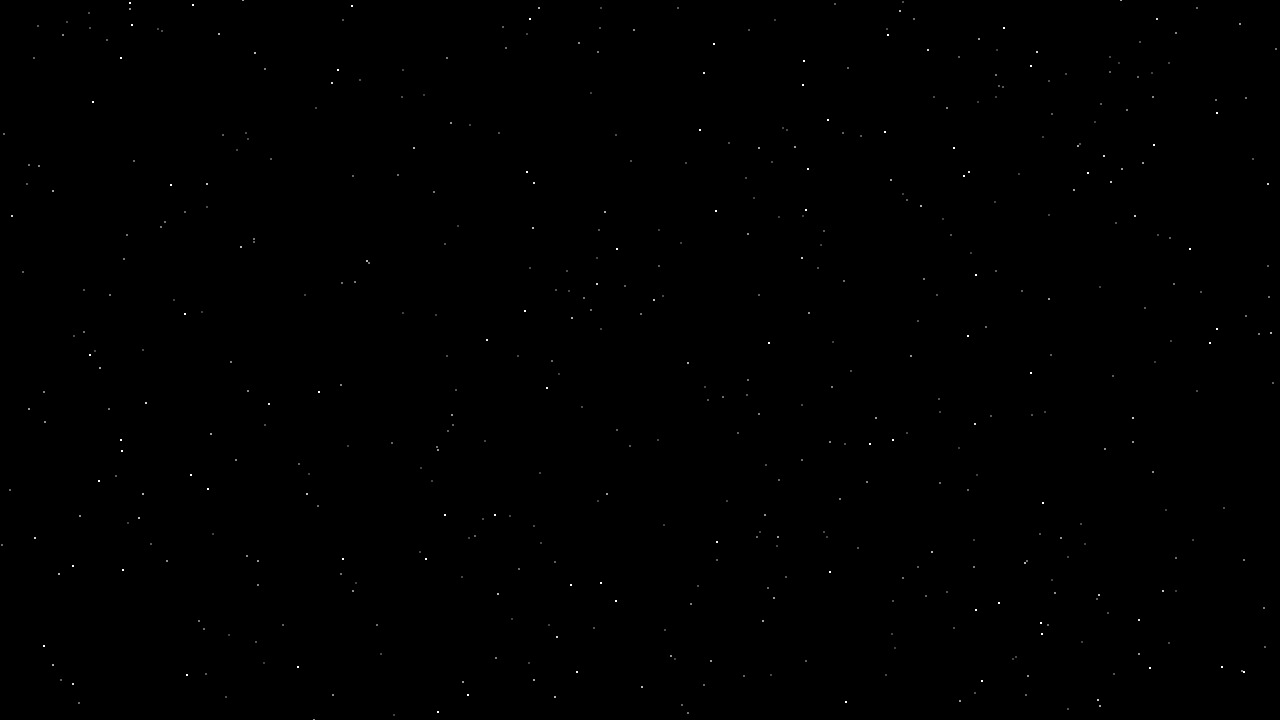
\includegraphics[width=12cm]{distancecolor.png}
\caption{Moving stars (we promise!) colored by their distance from the camera}
\end{center}
\end{figure}
\vspace{-0.5cm}

\noindent
When it came time to write this document (quite some time after implementing the things shown above)
we went back to the code and finally added motion blur. Mikael had already experimented with
doing so, and had written a somewhat functional variant that added trails by
''rewinding'' the motion of each star (by applying negative velocity) some fixed number of times.
This caused the stars to show broken trails at high velocities (and, looking at the picture,
something seems off about the brightness as well):

\begin{figure}[H]
\begin{center}
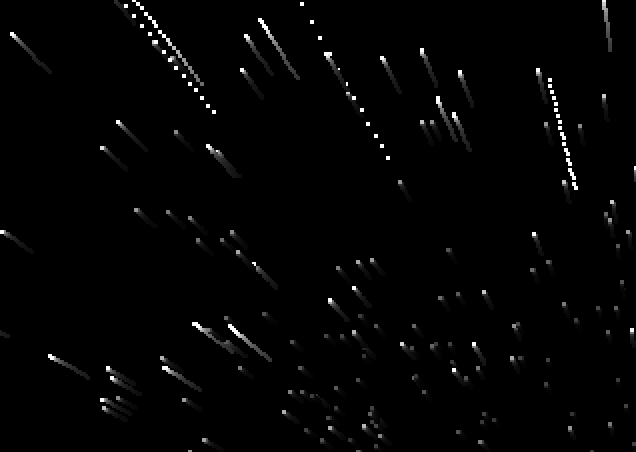
\includegraphics[width=7cm]{lurblurtrails.png}
\caption{Early motion blur attempt with broken trails}
\end{center}
\end{figure}
\vspace{-0.5cm}

\noindent
With our experience from the later labs in general and the use of linear interpolation in
particular we reimplemented motion blur by, for each star, interpolating a line between the
current position of the star and a point some set distance behind (in $z$) the star. We then interpolate
a color gradient going from black to the distance-based brightness, using the same number of steps
as there are pixels in the line. Finally we simply draw each pixel of the line using the color
of the corresponding index in the gradient vector.

\begin{figure}[H]
\begin{center}
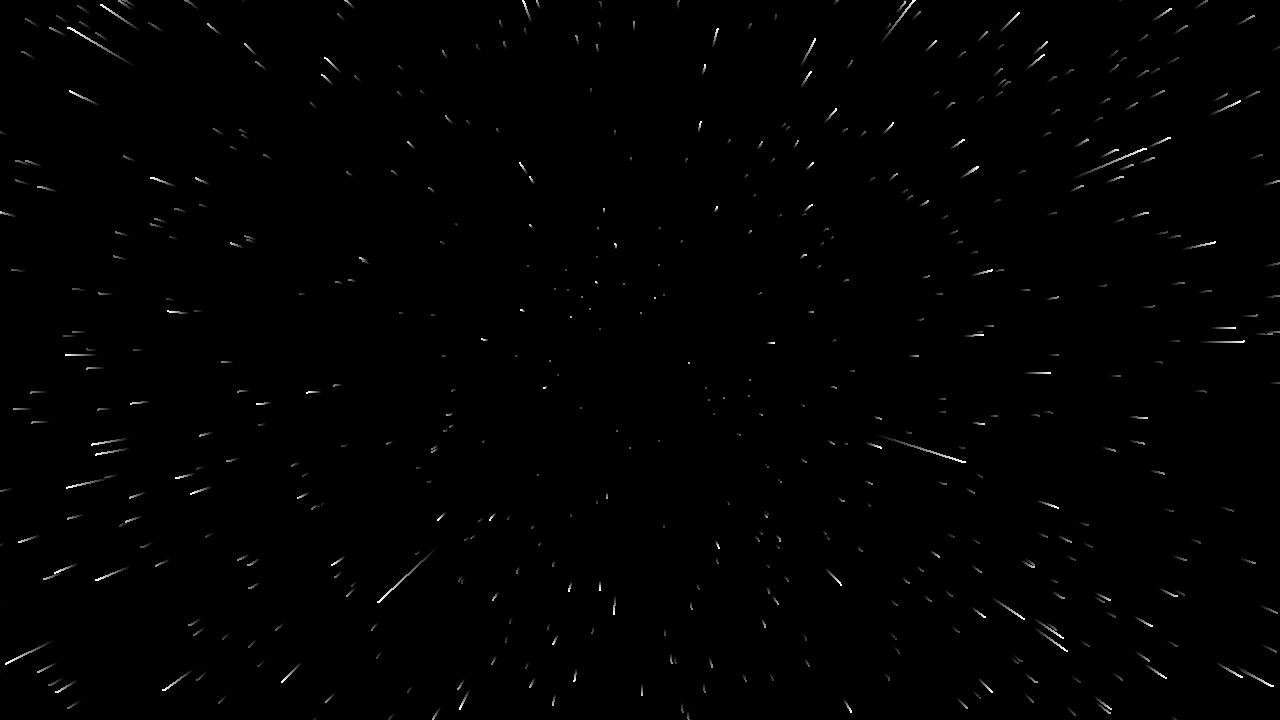
\includegraphics[width=12cm]{motionblur.png}
\caption{Final motion blur}
\end{center}
\end{figure}
\vspace{-0.5cm}

\section*{Contributions}
This lab mostly consisted of simply following the given instructions. The only area where it is
meaningful to discuss individual contributions is the motion blur. Mikael wrote the code for the
final motion blur, and when mentioning that he was doing so Robin spontaneously suggested the exact
technique that Mikael was already using.

\end{document}
